\documentclass[twocolumn]{article}

\usepackage{listings}										
\usepackage{graphicx}									

\title{Assignment #2\\Computational Physics I - Phys381}		
\author{Guilherme Contesini , 10140201}		

\begin{document}
\onecolumn{
\maketitle
\date
\begin{abstract} \textbf{'Title'} \newline

\end{abstract} 
}
\twocolumn
\newpage														

%%%%%%%%%%%%%%%%%%%%%%%%%%%%%%%%%%%%%%%%%%%%%%%%%%%%%%%%%%%%%%%%%%%%%%%%%%%%%%%%%%%%%%%%%%%%%%%%%%%%%%%%%%%%%%%%%%%%%%%%
\section{Introduction} 
%%%%%%%%%%%%%%%%%%%%%%%%%%%%%%%%%%%%%%%%%%%%%%%%%%%%%%%%%%%%%%%%%%%%%%%%%%%%%%%%%%%%%%%%%%%%%%%%%%%%%%%%%%%%%%%%%%%%%%%%
\section{Errors in computation}													
%%%%%%%%%%%%%%%%%%%%%%%%%%%%%%%%%%%%%%%%%%%%%%%%%%%%%%%%%%%%%%%%%%%%%%%%%%%%%%%%%%%%%%%%%%%%%%%%%%%%%%%%%%%%%%%%%%%%%%%%
\subsection{Calculation of $π$}													
%%%%%%%%%%%%%%%%%%%%%%%%%%%%%%%%%%%%%%%%%%%%%%%%%%%%%%%%%%%%%%%%%%%%%%%%%%%%%%%%%%%%%%%%%%%%%%%%%%%%%%%%%%%%%%%%%%%%%%%%
\subsubsection{(i)}
The Fortran code can be found in the Appendix Section \ref{[Madhava algorithm]}							
%%%%%%%%%%%%%%%%%%%%%%%%%%%%%%%%%%%%%%%%%%%%%%%%%%%%%%%%%%%%%%%%%%%%%%%%%%%%%%%%%%%%%%%%%%%%%%%%%%%%%%%%%%%%%%%%%%%%%%%%
\subsubsection{(ii)}			
\begin{figure}[!h]
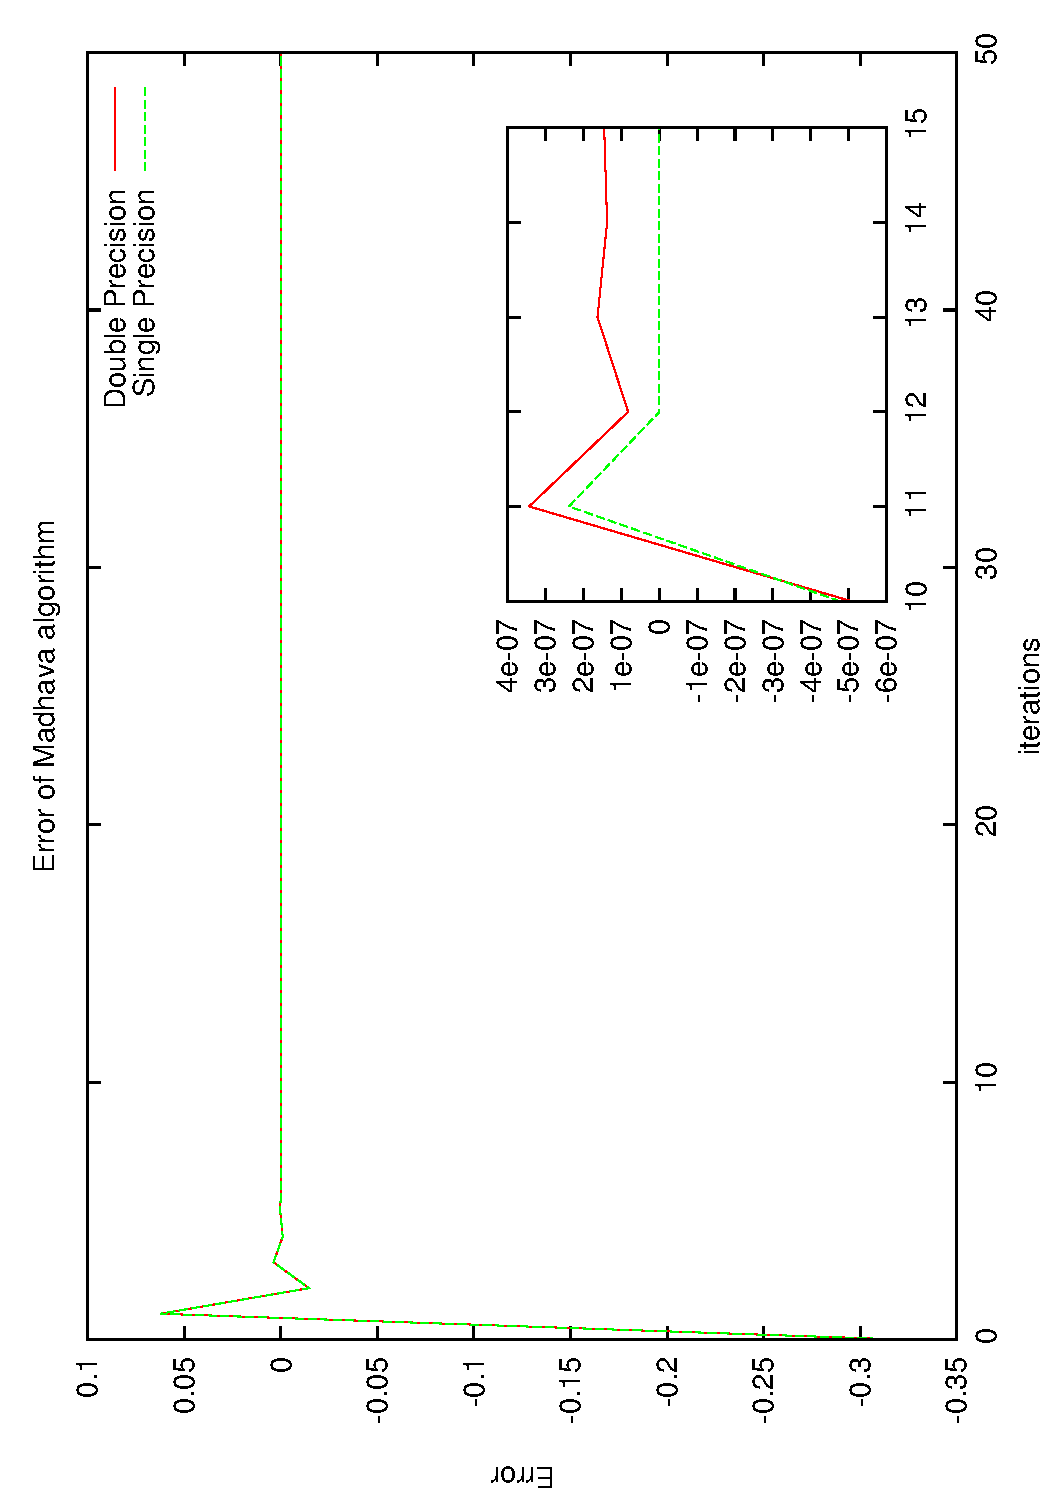
\includegraphics[width=2.in\textwidth, angle=270]{ErrorofMadhavaalgorithm.pdf}
\caption{The caption goes here}
\end{figure}

										
%%%%%%%%%%%%%%%%%%%%%%%%%%%%%%%%%%%%%%%%%%%%%%%%%%%%%%%%%%%%%%%%%%%%%%%%%%%%%%%%%%%%%%%%%%%%%%%%%%%%%%%%%%%%%%%%%%%%%%%%
\subsubsection{(iii)}													
%%%%%%%%%%%%%%%%%%%%%%%%%%%%%%%%%%%%%%%%%%%%%%%%%%%%%%%%%%%%%%%%%%%%%%%%%%%%%%%%%%%%%%%%%%%%%%%%%%%%%%%%%%%%%%%%%%%%%%%%
\section{Conclusion} 												
%%%%%%%%%%%%%%%%%%%%%%%%%%%%%%%%%%%%%%%%%%%%%%%%%%%%%%%%%%%%%%%%%%%%%%%%%%%%%%%%%%%%%%%%%%%%%%%%%%%%%%%%%%%%%%%%%%%%%%%%
\section{Appendix Codes:}
%%%%%%%%%%%%%%%%%%%%%%%%%%%%%%%%%%%%%%%%%%%%%%%%%%%%%%%%%%%%%%%%%%%%%%%%%%%%%%%%%%%%%%%%%%%%%%%%%%%%%%%%%%%%%%%%%%%%%%%%
\subsection{Madhava algorithm-(ii)}\label{[Madhava algorithm]}
\begin{verbatim}\caption{The caption goes here}
program indian_pi
  implicit none
  double precision :: my_pi_dp , 
  real_pi_dp , sum_dp , pi_dp
  real :: sum_float , my_pi_float , 
pi_float
  integer :: i_int
  open(12,file="pi_error.txt",action=
"write")
  pi_dp = 3.141592653589793
  pi_float = 3.141592653589793
  sum_dp = 0.
  sum_float = 0.
  do i_int = 0,50,1
    sum_dp = (((-1.)**(i_int))/(((2.*
    i_int)+1)*(3.**i_int))) + sum_dp

    sum_float = (((-1.)**(i_int))/
    (((2.*i_int)+1)*(3.**i_int))) 
    + sum_float

    my_pi_dp = sqrt(12.)*sum_dp
    my_pi_float = sqrt(12.)*sum_float
    write(12,*)i_int , (pi_float-
    my_pi_float) , (pi_dp-my_pi_dp)
  end do
  close(12)
end program
\end{verbatim}
%%%%%%%%%%%%%%%%%%%%%%%%%%%%%%%%%%%%%%%%%%%%%%%%%%%%%%%%%%%%%%%%%%%%%%%%%%%%%%%%%%%%%%%%%%%%%%%%%%%%%%%%%%%%%%%%%%%%%%%%

%%%%%%%%%%%%%%%%%%%%%%%%%%%%%%%%%%%%%%%%%%%%%%%%%%%%%%%%%%%%%%%%%%%%%%%%%%%%%%%%%%%%%%%%%%%%%%%%%%%%%%%%%%%%%%%%%%%%%%%%
\end{document}